\documentclass{beamer}

\usepackage[utf8]{inputenc}
\usepackage{verbatim}
\usepackage{bm} % for correct font and emphasis in formulation max/min
\usepackage{multirow}
\usepackage{booktabs} % for cmidrule
\usepackage[normalem]{ulem} % for "sout" that is strikeout
\newcommand{\tilderange}{\raisebox{0.5ex}{\texttildelow}}

% For ignoring margins in slides.
\newcommand\Wider[2][3em]{%
\makebox[\linewidth][c]{%
  \begin{minipage}{\dimexpr\textwidth+#1\relax}
  \raggedright#2
  \end{minipage}%
  }%
}

% Necessary for formulation layout workaround.
\newcommand{\pushright}[0]{\hskip \textwidth minus \textwidth}
\makeatletter
\newcommand{\specialcell}[1]{\ifmeasuring@#1\else\omit$\displaystyle#1$\ignorespaces\fi}

\AtBeginSection[]
{
  \begin{frame}[noframenumbering,plain]
    \frametitle{Outline for ``\currentsection''}
    \tableofcontents[
    currentsubsection,
    hideothersubsections,
    sectionstyle=show/shaded
    ]
  \end{frame}
}

% Allows for refering to the current section name
\newcommand{\currentsection}{}
\newcommand{\mysection}[1]{\renewcommand{\currentsection}{#1}\section{#1}}

\beamertemplateballitem
\usetheme{Antibes}
	\usecolortheme[RGB={120,0,0}]{structure}
	\setbeamertemplate{blocks}[rounded][shadow=true]
%\setbeamertemplate{footline}{\insertframenumber/\inserttotalframenumber}
	\setbeamerfont{page number in head/foot}{size=\large}
	\setbeamertemplate{footline}[frame number]
	\setbeamercovered{transparent=5}
	\setbeamertemplate{navigation symbols}{}
	% To number the references.
	\setbeamertemplate{bibliography item}{\insertbiblabel}

% used to avoid counting references as extra slides
\newcommand{\backupbegin}{
   \newcounter{framenumberappendix}
   \setcounter{framenumberappendix}{\value{framenumber}}
}
\newcommand{\backupend}{
   \addtocounter{framenumberappendix}{-\value{framenumber}}
   \addtocounter{framenumber}{\value{framenumberappendix}}
}

\usepackage{algorithm}
\usepackage[noend]{algpseudocode}

\newcommand{\dslidefs}{\footnotesize}

\usepackage{tikz}
\usetikzlibrary{patterns}
% Define transparent elements
\setbeamercovered{invisible}
\newcommand{\semitransp}[2][35]{\color{fg!#1}#2\color{fg!100}}
\newcommand{\drawhvector}[5]{
	\edef \origin {#1}
	\edef \xmax {#2}
	\edef \rs {(#3,#4)}
	\edef \scale {#5}
	\foreach \x in {0,...,\xmax}{
		\draw [shift={\origin}] (\x,0) rectangle +\rs;
		\node [scale=\scale, shift={\origin}, font=\LARGE] at (\x + 0.5, 0.5) {\(\x\)};
	}
}
\newcommand{\drawhvectornotext}[5]{
	\edef \origin {#1}
	\edef \xmax {#2}
	\edef \rs {(#3,#4)}
	\edef \scale {#5}
	\foreach \x in {0,...,\xmax}{
		\draw [shift={\origin}] (\x,0) rectangle +\rs;
		%\node [scale=\scale, shift={\origin}, font=\LARGE] at (\x + 0.5, 0.5) {\(\x\)};
	}
}
\newcommand{\drawhvectorfill}[6]{
	\edef \origin {#1}
	\edef \xmax {#2}
	\edef \rs {(#3,#4)}
	\edef \scale {#5}
	\edef \filling {#6}
	\foreach \x in {0,...,\xmax}{
		\draw [shift={\origin},fill=\filling] (\x,0) rectangle +\rs;
		%\node [scale=\scale, shift={\origin}, font=\LARGE] at (\x + 0.5, 0.5) {\(\x\)};
	}
}
\newcommand{\drawaxis}[2]{
	\edef \xmax {#1}
	\edef \ymax {#2}
	\draw [<->, thick] (\xmax,0) -- (0,0) -- (0,\ymax);
	\node [below, font=\small] at (\xmax/2, 0) {weight};
	\node [rotate=90, above, font=\small] at (0,\xmax/2) {profit};
}
\newcommand{\dominate}[3]{
	\edef \xx {#1}
	\edef \yy {#2}
	\edef \xmax {#3}
	\draw [dashed] (\xx, 0) -- (\xx,\yy) -- (\xmax,\yy);
}

% 12-color safe palette for color blindness
% http://mkweb.bcgsc.ca/colorblind/palettes.mhtml#page-container
\definecolor{jam}{RGB}{159,1,98}
\definecolor{creepers}{RGB}{0,159,129}
\definecolor{barbie}{RGB}{255,90,175}
\definecolor{aquamarine}{RGB}{0,252,207}
\definecolor{french}{RGB}{132,0,205}
\definecolor{dodger}{RGB}{0,141,249}
\definecolor{capri}{RGB}{0,194,249}
\definecolor{plum}{RGB}{255,178,253}
\definecolor{carmine}{RGB}{164,1,34}
\definecolor{crimson}{RGB}{226,1,52}
\definecolor{outragerous}{RGB}{255,110,58}
\definecolor{spark}{RGB}{255,195,59}

\newcommand{\stkout}[1]{\ifmmode\text{\sout{\ensuremath{#1}}}\else\sout{#1}\fi}
\definecolor{sameasbeforegray}{gray}{0.45}
\colorlet{notanymorecolor}{crimson}
\colorlet{newthingcolor}{creepers}
\newcommand\notanymore[1]{\textcolor{notanymorecolor}{\stkout{#1}}}
\newcommand\sameasbefore[1]{\textcolor{sameasbeforegray}{#1}}
\newcommand\newthing[1]{\textcolor{newthingcolor}{#1}}

\definecolor{bronze}{HTML}{a77044}
\definecolor{silver}{HTML}{71706C}
\definecolor{gold}{HTML}{d6af36}
\colorlet{originalcolor}{bronze}
\colorlet{faithfulcolor}{silver}
\colorlet{enhancedcolor}{gold}

% Change the spacing in a 'table of contents'/outline
\usepackage{etoolbox} % allows patching macros
\makeatletter
\patchcmd{\beamer@sectionintoc}{\vskip1.5em}{\vskip0.5em}{}{}
\makeatother

\newif\ifplacelogo % flag to disable logo
\placelogotrue % displays logo unless set to false

\begin{document}

\title{The state of the art in MILP formulations for the guillotine 2D knapsack and related problems}
\author{Henrique Becker\\[2\baselineskip] \small Advisor: Luciana S. Buriol\\Co-Advisor: Olinto Araújo}
\logo{\ifplacelogo
\includegraphics[scale=0.2]{inf}\fi}
\date{Friday, July 8, 2022}

{
	\setbeamertemplate{footline}{}
	\begin{frame}[noframenumbering]
	\titlepage
	\end{frame}
}

% LAST THING TODO: create a list of topics and copy it between each section
{
	\setbeamertemplate{footline}{}
	\begin{frame}[noframenumbering]
	\frametitle{Outline}
	\tableofcontents[hideallsubsections]
	\end{frame}
}

% Colors: jam, creepers, barbie, aquamarine, french, dodger, capri, plum,
% carmine, crimson, outragerous, spark

\mysection{Introduction}
\subsection{The Problem}
\frame{\frametitle{Objective Function}
\center
The Guillotine 2D Knapsack Problem (G2KP) maximizes the profit obtained from cutting pieces from a single large `original plate'.

\def\kx{0.200}
\def\ky{0}
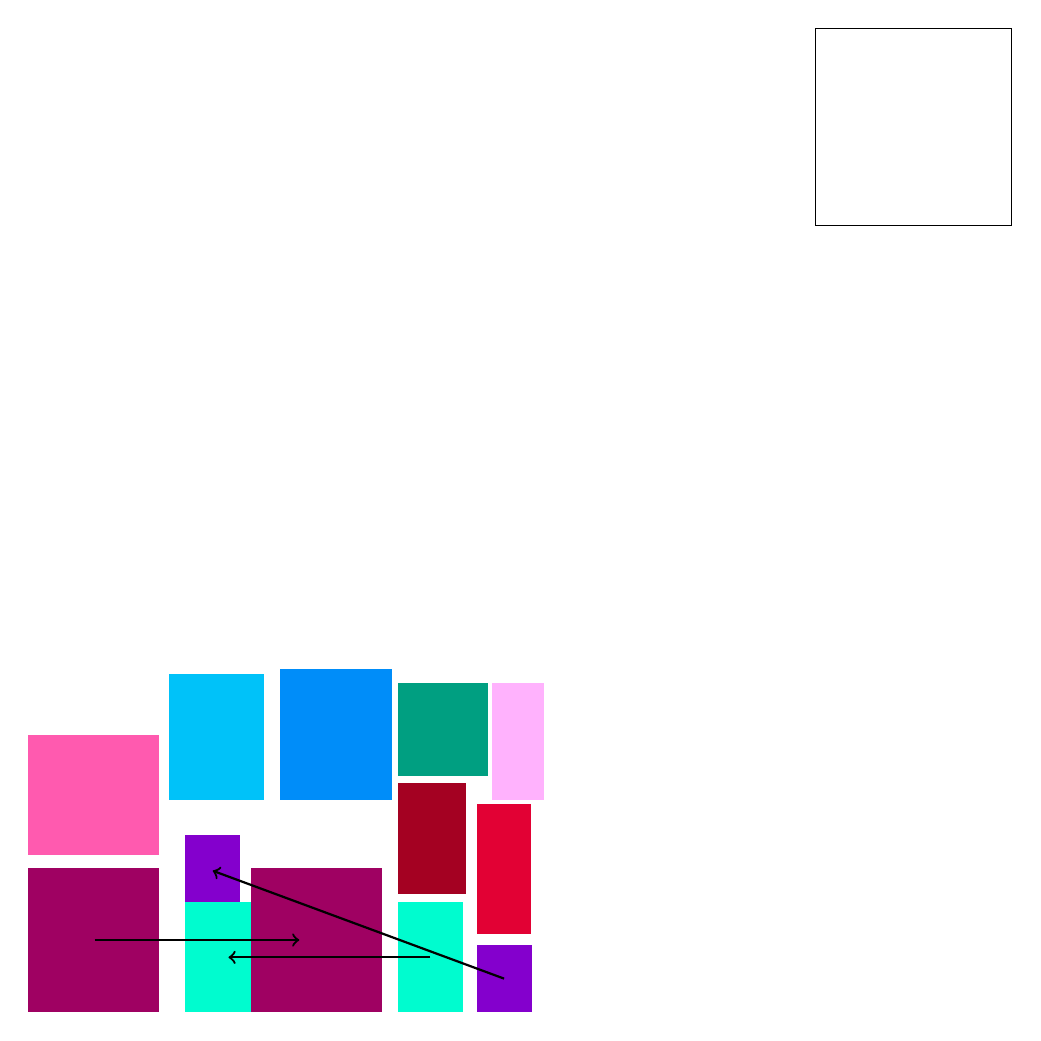
\begin{tikzpicture}[scale=10]

\fill[aquamarine] (0.470,0) rectangle +(0.083, 0.140);
\onslide<3-4>{\fill[aquamarine] (0.200,0) rectangle +(0.083, 0.140);}

\fill[french] (0.570,0) rectangle +(0.070, 0.086);
\onslide<3-4>{\fill[french] (0.200,0.140) rectangle +(0.070, 0.086);}

\fill[jam] (0,0) rectangle +(0.167, 0.184);
\onslide<3-4>{\fill[jam] (0.283,0) rectangle +(0.167, 0.184);}

\onslide<2-3>{\draw[thick,->] (0.605, 0.043) -- (0.235,0.180);} % french violet
\onslide<2-3>{\draw[thick,->] (0.511, 0.070) -- (0.255,0.070);} % aquamarine
\onslide<2-3>{\draw[thick,->] (0.085, 0.092) -- (0.345,0.092);} % jam

\fill[barbie] (0,0.200) rectangle +(0.167, 0.152);
\fill[creepers] (0.470,0.300) rectangle +(0.114, 0.118);
\fill[dodger] (0.320,0.270) rectangle +(0.143, 0.166);
\fill[capri] (0.180,0.270) rectangle +(0.120, 0.160);
\fill[plum] (0.590,0.270) rectangle +(0.066, 0.148);
\fill[carmine] (0.470,0.150) rectangle +(0.087, 0.141);
\fill[crimson] (0.570,0.10) rectangle +(0.069, 0.165);

\draw[black] ++(\kx, \ky) +(0,0) rectangle +(0.250, 0.250);
%\draw[dashed, thick, black] ++(\kx, \ky) +(0.083,0) -- +(0.083, 0.250);
%\draw[dashed, thick, black] ++(\kx, \ky) +(0,0.140) -- +(0.083, 0.140);
%\draw[dashed, thick, black] ++(\kx, \ky) +(0,0.226) -- +(0.083, 0.226);
%\draw[dashed, thick, black] ++(\kx, \ky) +(0.070,0.140) -- +(0.070, 0.250);
%\draw[dashed, thick, black] ++(\kx, \ky) +(0.083,0.184) -- +(0.250, 0.184);
\end{tikzpicture}
}

\frame{\frametitle{Guillotine Cuts}
\center
``every cut always go from one side of a plate to other; a cut never stops or starts from the middle of a plate''

\center
\def\kx{0.300}
\def\ky{0}
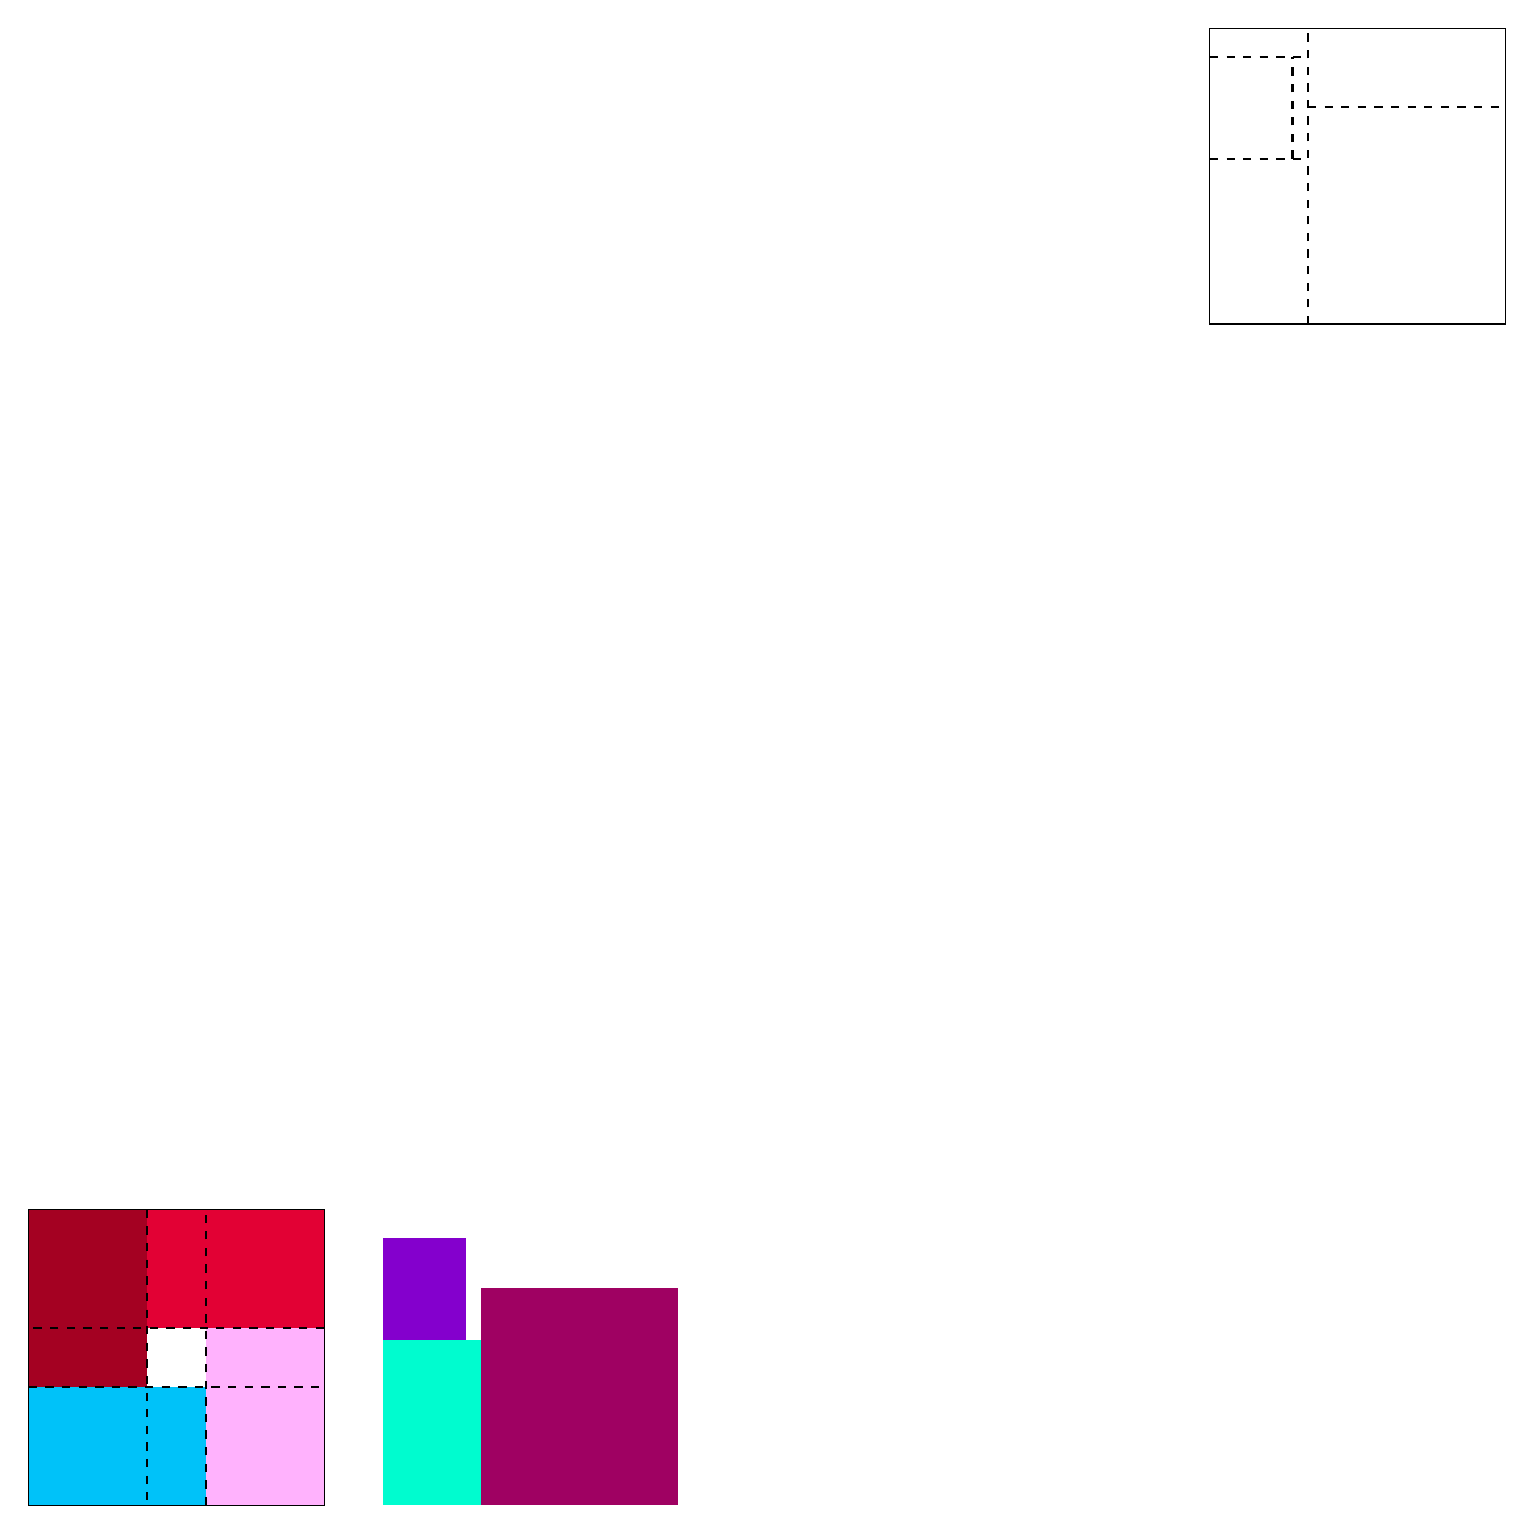
\begin{tikzpicture}[scale=15]

\fill[capri] (0, 0) rectangle +(0.150, 0.100);
\fill[plum] (0.150, 0) rectangle +(0.100, 0.150);
\fill[carmine] (0, 0.100) rectangle +(0.100, 0.150);
\fill[crimson] (0.100, 0.150) rectangle +(0.150, 0.100);
\draw[black] (0,0) rectangle +(0.250, 0.250);
\onslide<2>{\draw[dashed, thick, black] (0,0.100) -- (0.250, 0.100);}
\onslide<3>{\draw[dashed, thick, black] (0.150,0) -- (0.150, 0.250);}
\onslide<4>{\draw[dashed, thick, black] (0.250, 0.150) -- (0.,0.150);}
\onslide<5>{\draw[dashed, thick, black] (0.100,0.250) -- (0.100, 0.0);}

\fill[aquamarine] (0.300,0) rectangle +(0.083, 0.140);
\fill[french] (0.300,0.140) rectangle +(0.070, 0.086);
\fill[jam] (0.383,0) rectangle +(0.167, 0.184);
\draw[black] ++(\kx, \ky) +(0,0) rectangle +(0.250, 0.250);
\onslide<2->{\draw[dashed, thick, black] ++(\kx, \ky) +(0.083,0) -- +(0.083, 0.250);}
\onslide<3->{\draw[dashed, thick, black] ++(\kx, \ky) +(0,0.140) -- +(0.083, 0.140);}
\onslide<4->{\draw[dashed, thick, black] ++(\kx, \ky) +(0,0.226) -- +(0.083, 0.226);}
\onslide<5->{\draw[dashed, thick, black] ++(\kx, \ky) +(0.070,0.140) -- +(0.070, 0.226);}
\onslide<6>{\draw[dashed, thick, black] ++(\kx, \ky) +(0.083,0.184) -- +(0.250, 0.184);}
\end{tikzpicture}
}

\frame{\frametitle{Orthogonal Cuts and Non-Orthogonal (Irregular) Cuts}
\center
``\emph{Orthogonal cuts} are always parallel to one side of a plate (and perpendicular to the other).''

\center
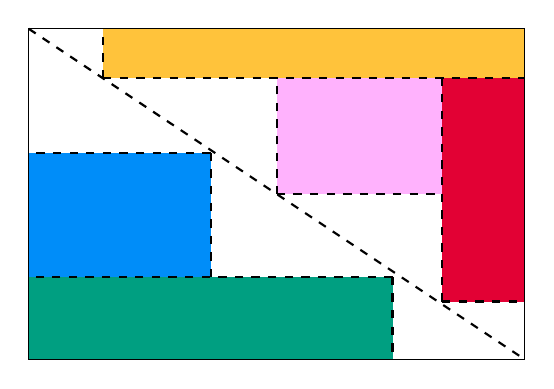
\begin{tikzpicture}[scale=21]

\fill[creepers] (0,0) rectangle +(0.220, 0.050);
\fill[dodger] (0,0.050) rectangle +(0.110, 0.075);
\fill[spark] (0.045,0.170) rectangle +(0.255, 0.030);
\fill[crimson] (0.250,0.035) rectangle +(0.050, 0.135);
\fill[plum] (0.150, 0.100) rectangle +(0.100, 0.070);

\onslide<2->{\draw[dashed, thick, black] (0,0.200) -- (0.300, 0);} % diagonal

\onslide<3->{\draw[dashed, thick, black] (0.045,0.170) -- +(0, 0.030);} % before spark
\onslide<4->{\draw[dashed, thick, black] (0.045,0.170) -- +(0.255, 0.0);} % below spark

\onslide<5->{\draw[dashed, thick, black] (0.250,0.035) -- +(0, 0.135);} % before crimson
\onslide<6->{\draw[dashed, thick, black] (0.250,0.035) -- +(0.050, 0);} % below crimson

\onslide<7->{\draw[dashed, thick, black] (0.150,0.100) -- +(0, 0.070);} % before plum
\onslide<8->{\draw[dashed, thick, black] (0.150,0.100) -- +(0.100, 0);} % below plum

\onslide<9->{\draw[dashed, thick, black] (0.220,0.050) -- (0, 0.050);} % above creepers
\onslide<10->{\draw[dashed, thick, black] (0.220,0.050) -- (0.220, 0);} % after creepers

\onslide<11->{\draw[dashed, thick, black] (0.110,0.125) -- (0, 0.125);} % above dogder
\onslide<12->{\draw[dashed, thick, black] (0.110,0.125) -- (0.110, 0.050);} % after dodger

\draw[black] (0,0) rectangle +(0.300, 0.200);

\end{tikzpicture}
}

\frame{\frametitle{Unrestricted Cuts}
\center
\small``The position of a cut does not need to match a single piece dimension.''

\center
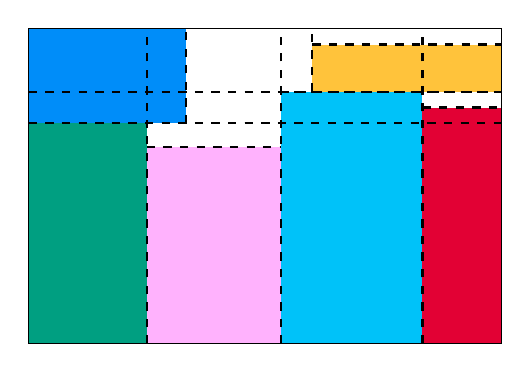
\begin{tikzpicture}[scale=20]

\fill[creepers] (0,0) rectangle +(0.075, 0.140);
\fill[plum] (0.075,0) rectangle +(0.085, 0.125);

\fill[capri] (0.160,0) rectangle +(0.090, 0.160);
\fill[crimson] (0.250,0) rectangle +(0.050, 0.150);

\fill[dodger] (0,0.140) rectangle +(0.100, 0.060);
\fill[spark] (0.180,0.160) rectangle +(0.120, 0.030);

\onslide<2>{\draw[dashed, thick, black] (0.075,0) -- (0.075, 0.200);}
\onslide<3>{\draw[dashed, thick, black] (0.250,0) -- (0.250, 0.200);}
\onslide<4>{\draw[dashed, thick, black] (0,0.140) -- (0.300, 0.140);}
\onslide<5>{\draw[dashed, thick, black] (0,0.160) -- (0.300, 0.160);}

\onslide<6->{\draw[dashed, thick, black] (0.160,0) -- (0.160, 0.200);} % first cut (between plum and capri)
\onslide<7->{\draw[dashed, thick, black] (0,0.140) -- (0.160, 0.140);} % between creepers and dodger
\onslide<8->{\draw[dashed, thick, black] (0.100,0.140) -- (0.100, 0.200);} % after dodger
\onslide<9->{\draw[dashed, thick, black] (0.075,0) -- (0.075, 0.140);} % between creepers and plum
\onslide<10->{\draw[dashed, thick, black] (0.075,0.125) -- (0.160, 0.125);} % above plum
\onslide<11->{\draw[dashed, thick, black] (0.160,0.160) -- (0.300, 0.160);} % below spark
\onslide<12->{\draw[dashed, thick, black] (0.250,0.0) -- (0.250, 0.160);} % between capri and crimson
\onslide<13->{\draw[dashed, thick, black] (0.250,0.150) -- (0.300, 0.150);} % above crimson
\onslide<14->{\draw[dashed, thick, black] (0.180,0.160) -- (0.180, 0.200);} % before spark
\onslide<15->{\draw[dashed, thick, black] (0.180,0.190) -- (0.300, 0.190);} % below spark

\draw[black] (0,0) rectangle +(0.300, 0.200);
\end{tikzpicture}
}

\frame{\frametitle{Constrained Demand}
\center
``There is a limit on the number of copies a piece may be sold.''

\def\kx{0.350}
\def\ky{0}
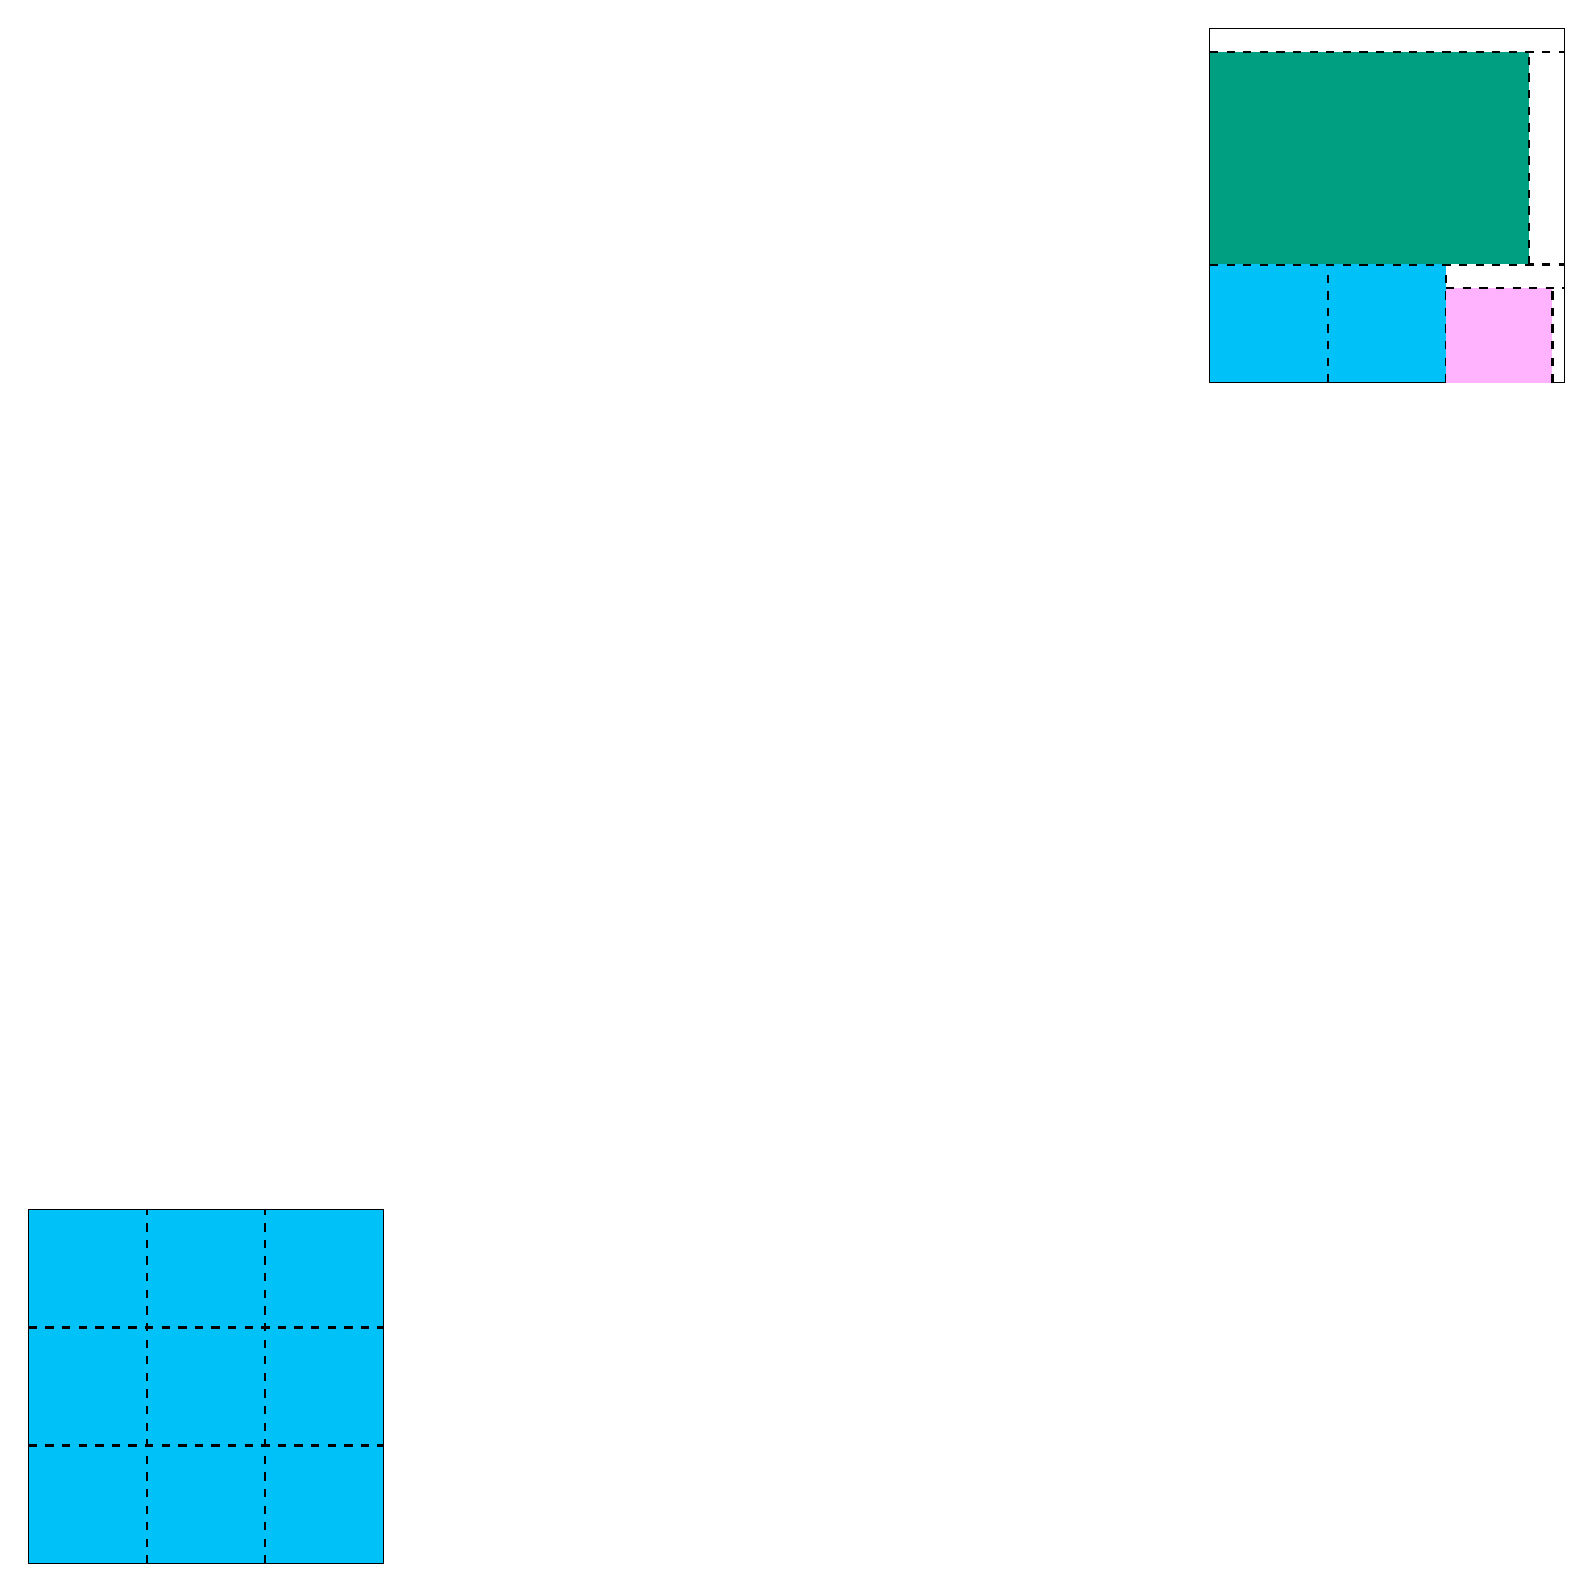
\begin{tikzpicture}[scale=15]
% First Plate
\fill[capri] (0, 0) rectangle +(0.300, 0.300);
\draw[black] (0,0) rectangle +(0.300, 0.300);
\draw[dashed, thick, black] (0,0.100) -- (0.300, 0.100);
\draw[dashed, thick, black] (0,0.200) -- (0.300, 0.200);
\draw[dashed, thick, black] (0.100,0) -- (0.100, 0.300);
\draw[dashed, thick, black] (0.200,0) -- (0.200, 0.300);

% Second Plate
\fill[capri] ++(\kx, \ky) +(0, 0) rectangle +(0.200, 0.100);
\draw[black] ++(\kx, \ky) +(0,0) rectangle +(0.300, 0.300);
\draw[dashed, thick, black] ++(\kx, \ky) +(0,0.100) -- +(0.300, 0.100);
\draw[dashed, thick, black] ++(\kx, \ky) +(0.100,0) -- +(0.100, 0.100);
\draw[dashed, thick, black] ++(\kx, \ky) +(0.200,0) -- +(0.200, 0.100);

\fill[creepers] (\kx, \ky) ++(0, 0.100) rectangle +(0.270, 0.180);
\fill[plum] (\kx, \ky) ++(0.200, 0) rectangle +(0.090, 0.080);

\draw[dashed, thick, black] ++(\kx, \ky) +(0,0.280) -- +(0.300, 0.280);
\draw[dashed, thick, black] ++(\kx, \ky) +(0.270,0.100) -- +(0.270, 0.280);

\draw[dashed, thick, black] ++(\kx, \ky) +(0.200,0.080) -- +(0.300, 0.080);
\draw[dashed, thick, black] ++(\kx, \ky) +(0.290,0) -- +(0.290, 0.080);

\end{tikzpicture}
}

\frame{\frametitle{\(k\)-staged}
\center

{``In the exact \(k\)-staged G2KP, the guillotine is switched at most \(k-1\) times.''}

\def\kx{0}
\def\ky{0}

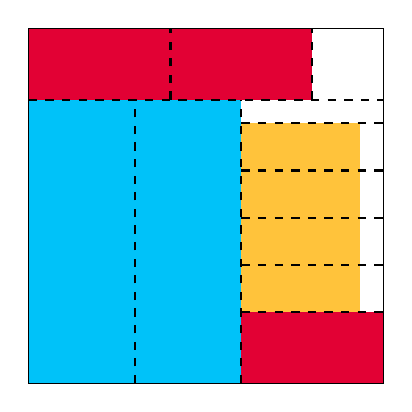
\begin{tikzpicture}[scale=15]

\onslide<3->{\fill[capri] (\kx, \ky) ++(0, 0) rectangle +(0.180, 0.240);}
\onslide<3->{\fill[crimson] (\kx, \ky) ++(0, 0.240) rectangle +(0.240, 0.060);}
\onslide<4->{\fill[crimson] (\kx, \ky) ++(0.180, 0) rectangle +(0.120, 0.060);}
\onslide<6->{\fill[spark] (\kx, \ky) ++(0.180, 0.060) rectangle +(0.100, 0.160);}
\draw[black] (\kx, \ky) ++(0,0) rectangle +(0.300, 0.300);

\onslide<2->{\draw[dashed, thick, black] ++(\kx, \ky) +(0,0.240) -- +(0.300, 0.240);} % first cut

\onslide<3->{\draw[dashed, thick, black] ++(\kx, \ky) +(0.120,0.240) -- +(0.120, 0.300);} % vertical top cuts
\onslide<3->{\draw[dashed, thick, black] ++(\kx, \ky) +(0.240,0.240) -- +(0.240, 0.300);} % vertical top cuts
\onslide<3->{\draw[dashed, thick, black] ++(\kx, \ky) +(0.090,0) -- +(0.090, 0.240);} % vertical bottom cuts
\onslide<3->{\draw[dashed, thick, black] ++(\kx, \ky) +(0.180,0) -- +(0.180, 0.240);} % vertical bottom cuts

\onslide<5->{\draw[dashed, thick, black] ++(\kx, \ky) +(0.180,0.060) -- +(0.300, 0.060);} % third stage cuts
\onslide<6->{\draw[dashed, thick, black] ++(\kx, \ky) +(0.180,0.100) -- +(0.300, 0.100);} % third stage cuts
\onslide<6->{\draw[dashed, thick, black] ++(\kx, \ky) +(0.180,0.140) -- +(0.300, 0.140);} % third stage cuts
\onslide<6->{\draw[dashed, thick, black] ++(\kx, \ky) +(0.180,0.180) -- +(0.300, 0.180);} % third stage cuts
\onslide<6->{\draw[dashed, thick, black] ++(\kx, \ky) +(0.180,0.220) -- +(0.300, 0.220);} % third stage cuts

\end{tikzpicture}

\onslide<4->{\small ``The non-exact \(k\)-staged G2KP adds one extra stage in which the only cuts allowed are the ones that trim plates to the size of pieces''}
}

\frame{\frametitle{Allow or disallow rotation}
\center
We may allow (or not) for pieces/plates to switch length and width (i.e., 90 degree rotations).
% NOTE: as we only allow orthogonal cuts the only allowed rotation is 90 degrees, and there is at most two different representations of a piece (squares just have one).

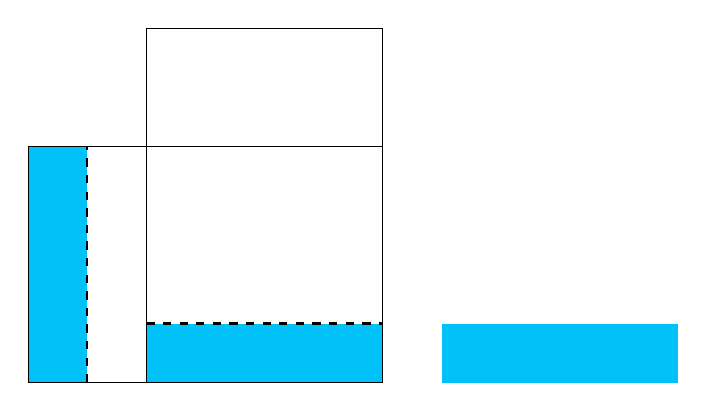
\begin{tikzpicture}[scale=15]

\fill[capri] (0.350, 0) rectangle +(0.200, 0.050); % piece out

\onslide<2>{\fill[capri] (0, 0) rectangle +(0.050, 0.200);} % piece in (first)
\onslide<2>{\draw[dashed, thick, black]  (0.050,0) -- (0.050, 0.200);} % cut (first)
\onslide<1-2>{\draw[black] (0,0) rectangle +(0.300, 0.200);} % plate (first)

\onslide<3>{\fill[capri] (0.100, 0) rectangle +(0.200, 0.050);} % piece in (second)
\onslide<3>{\draw[dashed, thick, black] (0.100,0.050) -- (0.300, 0.050);} % cut (second)
\onslide<3>{\draw[black] (0.100,0) rectangle +(0.200, 0.300);} % plate (second)

\end{tikzpicture}
}

\frame{\frametitle{Summary of the G2KP characteristics}
\begin{itemize}
\item Knapsack -- maximises profit, single plate.
\item Guillotine Cuts -- from a side to another.
\item Orthogonal Cuts -- only cuts parallel to the sides.
\item Unrestricted Cuts -- may cut in any position.
\item Constrained Demand -- upper bound for pieces in solution.
\item Unlimited Stages -- no limit on cut orientation changes.
\item Allow/disallow rotation -- of pieces or plates.
\end{itemize}
}


\mysection{Prior Work}
\subsection{Seminal Works and Surveys}
\begin{frame}[t]{Seminal Works and Surveys}
\setbeamercovered{transparent=50}
\begin{description}
% gg:65 (first version of unconstrained weakly NP-Hard)
% herz:72 (unconstrained seminal work, introduces cut enumeration)
% cw7 (constrained exact seminal work, introduces cut enumeration)
% iori:2020
% russo:2020
\item<1-1>[1965] Introduces the unconstrained (weakly NP-Hard) G2KP and other variants (no experiments). \alt<1-1>{\alert{\cite{gg:1965}}}{\cite{gg:1965}}
\item<2-2>[1972] Seminal work on the unconstrained G2KP. Introduces `canonical dissecations' (used pervasively).\alt<2-2>{\alert{\cite{herz:1972}}}{\cite{herz:1972}}
\item<3-3>[1977] Seminal work on the constrained G2KP. Treats some symmetries. Proposes classical instances.\alt<3-3>{\alert{\cite{cw:1977}}}{\cite{cw:1977}}
\item<4-4>[2020] Surveys exact methods and relaxations on 2D cutting and packing. \alt<4-4>{\alert{\cite{iori:2020}}}{\cite{iori:2020}}
\item<5-5>[2020] Surveys exact methods and relaxations the G2KP specifically; points out mistakes in the literature. \alt<5-5>{\alert{\cite{russo:2020}}}{\cite{russo:2020}}
\end{description}
\only<1-1>{\alert{\cite{gg:1965}} Gilmore, P. C.; Gomory, R. E. Multistage Cutting Stock Problems of Two and More Dimensions. 10.1287/opre.13.1.94}
\only<2-2>{\alert{\cite{herz:1972}} Herz, J. C. Recursive Computational Procedure for Two-Dimensional Stock Cutting. 10.1147/rd.165.0462}
\only<3-3>{\alert{\cite{cw:1977}} Christofides, N.; Whitlock, C. An Algorithm for Two-Dimensional Cutting Problems. 10.1287/opre.25.1.30}
\only<4-4>{\alert{\cite{iori:2020}} Iori, M.; de Lima, V. L.; Martello, S.; Miyazawa, F. K.; Monaci, M. Exact Solution Techniques for Two-Dimensional Cutting and Packing. 10.1016/j.ejor.2020.06.050}
\only<5-5>{\alert{\cite{russo:2020}} Russo, M.; Boccia, M.; Sforza, A.; Sterle, C. Constrained Two-Dimensional Guillotine Cutting Problem: Upper-Bound Review and Categorization. 10.1111/itor.12687}
\end{frame}

\subsection{Formulations}
\begin{frame}{Formulations}
\setbeamercovered{transparent=50}
\begin{description}
\item<1-1>[2008] The first MILP formulation for unlimited stages. Mostly of theoretical interest. \alt<1-1>{\alert{\cite{messaoud:2008}}}{\cite{messaoud:2008}}
\item<2-2>[2010] Two- and (restricted) three-staged formulations for the G2CSP. Not the first \(k\)-staged formulation. \alt<2-2>{\alert{\cite{silva:2010}}}{\cite{silva:2010}}
\item<3-3>[2013] Compares three two-staged MILP formulations including the work mentioned above.\alt<3-3>{\alert{\cite{furini:2013}}}{\cite{furini:2013}}
\item<4-4>[2016] The first MILP formulation for the unlimited stages G2KP able to solve medium-sized intances.\alt<4-4>{\alert{\cite{furini:2016}}}{\cite{furini:2016}}
\item<5-5>[2020] Three new competitive formulations were proposed recently.\alt<5-5>{\alert{\cite{martin:2020:models}}}{\cite{martin:2020:models}}
\end{description}
\only<1-1>{\alert{\cite{messaoud:2008}} Ben Messaoud, S.; Chu, C.; Espinouse, M.-L. Characterization and Modelling of Guillotine Constraints. 10.1016/j.ejor.2007.08.029 }
\only<2-2>{\alert{\cite{silva:2010}} Silva, E.; Alvelos, F.; Valério de Carvalho, J. M. An Integer Programming Model for Two- and Three-Stage Two-Dimensional Cutting Stock Problems. 10.1016/j.ejor.2010.01.039 }
\only<3-3>{\alert{\cite{furini:2013}} Furini, F.; Malaguti, E. Models for the Two-Dimensional Two-Stage Cutting Stock Problem with Multiple Stock Size. 10.1016/j.cor.2013.02.026}
\only<4-4>{\alert{\cite{furini:2016}} Furini, F.; Malaguti, E.; Thomopulos, D. Modeling Two-Dimensional Guillotine Cutting Problems via Integer Programming. 10.1287/ijoc.2016.0710}
\only<5-5>{\alert{\cite{martin:2020:models}} Martin, M.; Morabito, R.; Munari, P. A Top-down Cutting Approach for Modeling the Constrained Two- and Three-Dimensional Guillotine Cutting Problems. 10.1080/01605682.2020.1813640.}

\end{frame}

\begin{frame}[fragile]
\frametitle{Current Work}
\centering
\begin{description}
%\item[(this thesis)] Old algorithms are implemented and tested. The influence of the datasets in the comparisons becomes apparent.
\item[(this work)] \begin{itemize}
\item enhances a state-of-the-art formulation by cutting down model size and symmetries;
\item adapts a previously known reduction to our context also reducing model size and symmetries;
\item brings new results for recently proposed and more challenging instances;
\item directly compares to the state of the art on MILP formulations for the problem;
\item adapts to related but distinct problems to further test the formulation;
\item proposes a hybridisation of the proposed model with a previous model for a restricted problem.
\end{itemize}
\end{description}
\end{frame}

\mysection{Reductions}
\subsection{Discretization}
\frame{\frametitle{Discretization}
\center
We can restrict cuts to linear combinations of piece dimensions (constrained by their demand) without losing optimality.

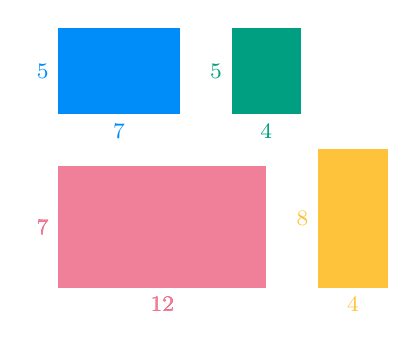
\begin{tikzpicture}[scale=22]
\fill[creepers] (0.10,0.10) rectangle +(0.04, 0.05);
\node[creepers] at (0.12, 0.10) [below]{\dslidefs 4};
\node[creepers] at (0.10, 0.125) [left]{\dslidefs 5};
\fill[dodger] (0,0.10) rectangle +(0.07, 0.05);
\node[dodger] at (0.035, 0.10) [below]{\dslidefs 7};
\node[dodger] at (0, 0.125) [left]{\dslidefs 5};
\fill[spark] (0.15,0) rectangle +(0.04, 0.08);
\node[spark] at (0.17, 0) [below]{\dslidefs 4};
\node[spark] at (0.15, 0.04) [left]{\dslidefs 8};
\onslide<-3>{
	\fill[crimson] (0,0) rectangle +(0.12, 0.07);
	\node[crimson] at (0.06, 0) [below]{\dslidefs 12};
	\node[crimson] at (0, 0.035) [left]{\dslidefs 7};
}
\onslide<4->{
	\fill[crimson!50] (0,0) rectangle +(0.12, 0.07);
	\node[crimson!50] at (0.06, 0) [below]{\dslidefs 12};
	\node[crimson!50] at (0, 0.035) [left]{\dslidefs 7};
}
\end{tikzpicture}
\hspace{0.25cm} % ----------------------------------------------------
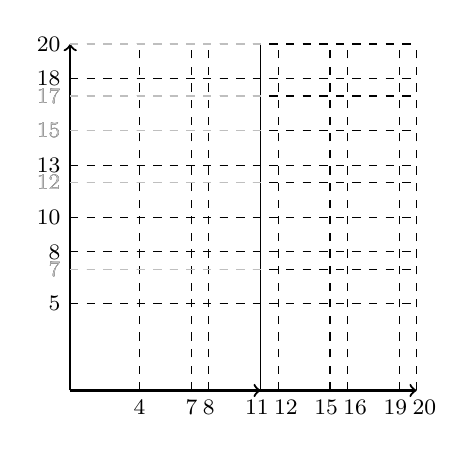
\begin{tikzpicture}[scale=22]
\draw[thick,->] (0, 0) -- (0,0.20); % y axis
\onslide<-2>{\draw[thick,->] (0, 0) -- (0.20,0);} % x axis
\onslide<3->{\draw[thick,->] (0, 0) -- (0.11,0);} % x axis

%left: 5, 7, 8, 10, 12, 13, 15, 17, 18, 20
\node at (0, 0.05) [left]{\dslidefs 5};
\onslide<-4>{\node at (0, 0.07) [left]{\dslidefs 7};}
\node at (0, 0.08) [left]{\dslidefs 8};
\node at (0, 0.10) [left]{\dslidefs 10};
\onslide<-4>{\node at (0, 0.12) [left]{\dslidefs 12};}
\node at (0, 0.13) [left]{\dslidefs 13};
\onslide<-4>{\node at (0, 0.15) [left]{\dslidefs 15};}
\onslide<-4>{\node at (0, 0.17) [left]{\dslidefs 17};}
\node at (0, 0.18) [left]{\dslidefs 18};
\node at (0, 0.20) [left]{\dslidefs 20};
\onslide<5>{\node[black!25] at (0, 0.07) [left]{\dslidefs 7};}
\onslide<5>{\node[black!25] at (0, 0.12) [left]{\dslidefs 12};}
\onslide<5>{\node[black!25] at (0, 0.15) [left]{\dslidefs 15};}
\onslide<5>{\node[black!25] at (0, 0.17) [left]{\dslidefs 17};}

% horizontal
\onslide<-2>{
	\draw[dashed, black] (0,0.05) -- (0.2, 0.05);
	\draw[dashed, black] (0,0.07) -- (0.2, 0.07);
	\draw[dashed, black] (0,0.08) -- (0.2, 0.08);
	\draw[dashed, black] (0,0.10) -- (0.2, 0.10);
	\draw[dashed, black] (0,0.12) -- (0.2, 0.12);
	\draw[dashed, black] (0,0.13) -- (0.2, 0.13);
	\draw[dashed, black] (0,0.15) -- (0.2, 0.15);
	\draw[dashed, black] (0,0.17) -- (0.2, 0.17);
	\draw[dashed, black] (0,0.18) -- (0.2, 0.18);
	\draw[dashed, black] (0,0.20) -- (0.2, 0.20);
}
\onslide<3->{
	\draw[dashed, black] (0,0.05) -- (0.11, 0.05);
	\draw[dashed, black] (0,0.07) -- (0.11, 0.07);
	\draw[dashed, black] (0,0.08) -- (0.11, 0.08);
	\draw[dashed, black] (0,0.10) -- (0.11, 0.10);
	\draw[dashed, black] (0,0.12) -- (0.11, 0.12);
	\draw[dashed, black] (0,0.13) -- (0.11, 0.13);
	\draw[dashed, black] (0,0.15) -- (0.11, 0.15);
	\draw[dashed, black] (0,0.17) -- (0.11, 0.17);
	\draw[dashed, black] (0,0.18) -- (0.11, 0.18);
	\draw[dashed, black] (0,0.20) -- (0.11, 0.20);
}

% below: 4, 7, 8, 11, 12, 15, 16, 19, 20
\node at (0.04, 0) [below]{\dslidefs 4};
\node at (0.07, 0) [below]{\dslidefs 7};
\node at (0.08, 0) [below]{\dslidefs 8};
\node at (0.11, 0) [below]{\dslidefs {11~~}};
\onslide<-2>{
\node at (0.12, 0) [below]{\dslidefs {~~12}};
\node at (0.15, 0) [below]{\dslidefs {15~~}};
\node at (0.16, 0) [below]{\dslidefs {~~16}};
\node at (0.19, 0) [below]{\dslidefs {19~~}};
\node at (0.20, 0) [below]{\dslidefs {~~20}};
}

% vertical
\draw[dashed, black] (0.04,0) -- (0.04, 0.2);
\draw[dashed, black] (0.07,0) -- (0.07, 0.2);
\draw[dashed, black] (0.08,0) -- (0.08, 0.2);
\draw[dashed, black] (0.11,0) -- (0.11, 0.2);
\onslide<-2>{
	\draw[dashed, black] (0.12,0) -- (0.12, 0.2);
	\draw[dashed, black] (0.15,0) -- (0.15, 0.2);
	\draw[dashed, black] (0.16,0) -- (0.16, 0.2);
	\draw[dashed, black] (0.19,0) -- (0.19, 0.2);
	\draw[dashed, black] (0.20,0) -- (0.20, 0.2);
}

\onslide<2>{\draw (0.11,0) -- (0.11, 0.2);}

\onslide<5>{
	\draw[dashed, black!25] (0,0.07) -- (0.11, 0.07);
	\draw[dashed, black!25] (0,0.12) -- (0.11, 0.12);
	\draw[dashed, black!25] (0,0.15) -- (0.11, 0.15);
	\draw[dashed, black!25] (0,0.17) -- (0.11, 0.17);
	\draw[dashed, black!25] (0,0.20) -- (0.11, 0.20);
}

\end{tikzpicture}
}

\subsection{Plate-Size Normalization}
\frame{\frametitle{Plate-Size Normalization I}
\center
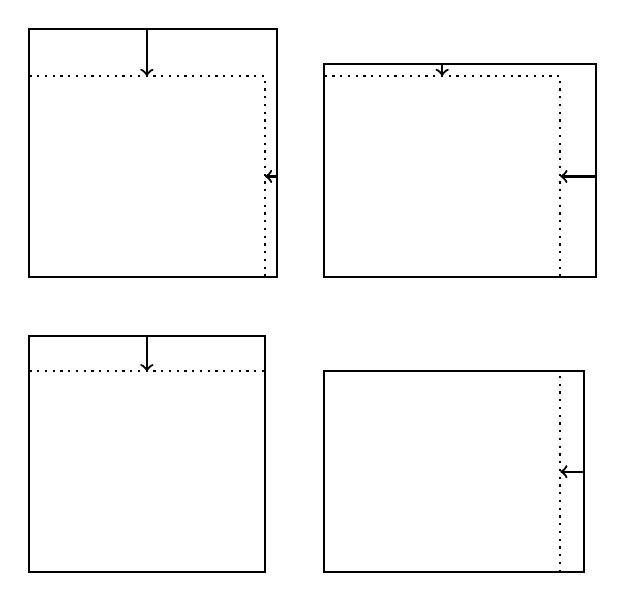
\begin{tikzpicture}[scale=15]
\draw[dotted, thick] (0, 0) rectangle +(0.20, 0.17);
\draw[black, thick] (0, 0) rectangle +(0.20, 0.20);
\draw[thick,->] (0.1, 0.20) -- (0.1,0.17);

\draw[dotted, thick] (0.25, 0) rectangle +(0.20, 0.17);
\draw[black, thick] (0.25, 0) rectangle +(0.22, 0.17);
\draw[thick,->] (0.47, 0.085) -- (0.45,0.085);

\draw[dotted, thick] (0, 0.25) rectangle +(0.20, 0.17);
\draw[black, thick] (0, 0.25) rectangle +(0.21, 0.21);
\draw[thick,->] (0.1, 0.46) -- (0.1,0.42);
\draw[thick,->] (0.21, 0.335) -- (0.20,0.335);

\draw[dotted, thick] (0.25, 0.25) rectangle +(0.20, 0.17);
\draw[black, thick] (0.25, 0.25) rectangle +(0.23, 0.18);
\draw[thick,->] (0.35, 0.43) -- (0.35,0.42);
\draw[thick,->] (0.48, 0.335) -- (0.45,0.335);

\end{tikzpicture}
}

\frame{\frametitle{Plate-Size Normalization II}
\centering
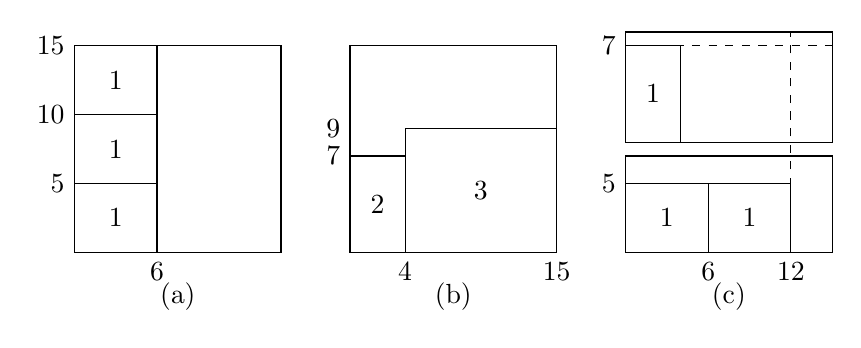
\begin{tikzpicture}[scale=0.175]
\begin{scope}[shift={(0, 0)}]
\draw [draw=black]   (0, 0) rectangle ++(15, 15);
\draw [draw=black]   (0, 0) rectangle     ++(6, 5) node [midway] {1};
\draw [draw=black]   (0, 5) rectangle     ++(6, 5) node [midway] {1};
\draw [draw=black] (0, 10) rectangle     ++(6, 5) node [midway] {1};
\node [left]  at (0, 5) {5};
\node [left]  at (0, 10) {10};
\node [left]  at (0, 15) {15};
\node [below]  at (6, 0) {6};
\node [below] at (7.5, -1.5) {(a)};
\end{scope}
\begin{scope}[shift={(20, 0)}]
\draw [draw=black]   (0, 0) rectangle ++(15, 15);
\draw [draw=black]   (0, 0) rectangle     ++(4, 7) node [midway] {2};
\draw [draw=black]   (4, 0) rectangle   ++(11, 9) node [midway] {3};
\node [below]  at   (4, 0)   {4};
\node [below]  at (15, 0) {15};
\node     [left]  at   (0, 7)   {7};
\node   [left]  at (0, 9)   {9};
\node [below] at (7.5, -1.5) {(b)};
\end{scope}
\begin{scope}[shift={(40, 0)}]
\draw [draw=black]   (0, 0) rectangle ++(15, 7);
\draw [draw=black]   (0, 0) rectangle     ++(6, 5) node [midway] {1};
\draw [draw=black]   (6, 0) rectangle     ++(6, 5) node [midway] {1};
\node [left]  at (0, 5) {5};
\node [below]  at (6, 0) {6};
\node [below]  at (12, 0) {12};
\draw[dashed] (12, 0) -- (12, 16);

\draw [draw=black]   (0, 8) rectangle ++(15, 8);
\draw [draw=black]   (0, 8) rectangle   ++(4, 7) node [midway] {1};

\node     [left]  at   (0, 15)   {7};
\draw [dashed] (0, 15) -- (15, 15);
\node [below] at (7.5, -1.5) {(c)};
\end{scope}
\end{tikzpicture}

}

% TODO: check if it is worth putting here a slide about other discretizations

\subsection{Previous Reductions}
\frame{\frametitle{Previous Reductions}
\begin{itemize}
%\item[(this thesis)] Old algorithms are implemented and tested. The influence of the datasets in the comparisons becomes apparent.
\item Redundant-Cut
\begin{itemize}
\item Remove unnecessary intermediary trim cuts.
\item Does not affect the number of plates (constraints).
\item Is superseded by our enhanced formulation.
\end{itemize}
\item Cut-Position
\begin{itemize}
\item Removes unrestricted cuts from small plates.
\item If 6 pieces do not fit, there is no loss.
\item Affects both number of variables and constraints.
\end{itemize}
\end{itemize}
% start with the one that links to the piece extraction symmetries
% "It is not a problem we had a proble reimplementing it because our enhanced model makes it obsolete."
% what is redundant-cut and cut position
}

\frame{\frametitle{Unrestricted Cuts (Revisited)}
\center
\small``The position of a cut does not need to match a single piece dimension.''

\center
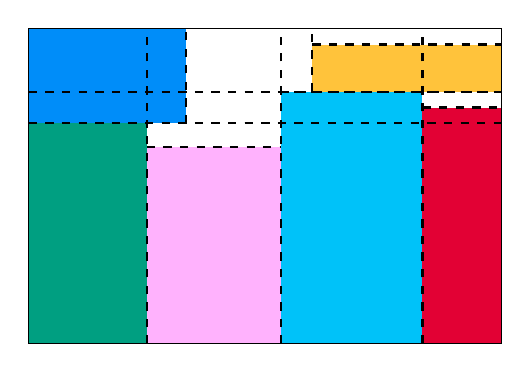
\begin{tikzpicture}[scale=20]

\fill[creepers] (0,0) rectangle +(0.075, 0.140);
\fill[plum] (0.075,0) rectangle +(0.085, 0.125);

\fill[capri] (0.160,0) rectangle +(0.090, 0.160);
\fill[crimson] (0.250,0) rectangle +(0.050, 0.150);

\fill[dodger] (0,0.140) rectangle +(0.100, 0.060);
\fill[spark] (0.180,0.160) rectangle +(0.120, 0.030);

\onslide<2>{\draw[dashed, thick, black] (0.075,0) -- (0.075, 0.200);}
\onslide<3>{\draw[dashed, thick, black] (0.250,0) -- (0.250, 0.200);}
\onslide<4>{\draw[dashed, thick, black] (0,0.140) -- (0.300, 0.140);}
\onslide<5>{\draw[dashed, thick, black] (0,0.160) -- (0.300, 0.160);}

\onslide<6->{\draw[dashed, thick, black] (0.160,0) -- (0.160, 0.200);} % first cut (between plum and capri)
\onslide<7->{\draw[dashed, thick, black] (0,0.140) -- (0.160, 0.140);} % between creepers and dodger
\onslide<8->{\draw[dashed, thick, black] (0.100,0.140) -- (0.100, 0.200);} % after dodger
\onslide<9->{\draw[dashed, thick, black] (0.075,0.125) -- (0.160, 0.125);} % above plum
\onslide<10->{\draw[dashed, thick, black] (0.075,0) -- (0.075, 0.140);} % between creepers and plum
\onslide<11->{\draw[dashed, thick, black] (0.160,0.160) -- (0.300, 0.160);} % below spark
\onslide<12->{\draw[dashed, thick, black] (0.250,0.0) -- (0.250, 0.160);} % between capri and crimson
\onslide<13->{\draw[dashed, thick, black] (0.250,0.150) -- (0.300, 0.150);} % above crimson
\onslide<14->{\draw[dashed, thick, black] (0.180,0.160) -- (0.180, 0.200);} % before spark
\onslide<15->{\draw[dashed, thick, black] (0.180,0.190) -- (0.300, 0.190);} % below spark

\draw[black] (0,0) rectangle +(0.300, 0.200);
\end{tikzpicture}
}
% repeat frame about restricted here

%\frame{\frametitle{Furini's Model}
%}
\mysection{Formulations}

\subsection{Furini's Formulation}
\frame{\frametitle{Furini's Formulation}
\begin{align*}
\bm{max.} & \sum_{j \textcolor{notanymorecolor}{\in \bar{J}}} p_j \textcolor{notanymorecolor}{y_j}\\
% UNFORTUNATELY, THE HSPACE BELOW MAY NEED MANUAL ADJUSTMENT
\bm{s.t.} & \specialcell{\textcolor{notanymorecolor}{y_j} \leq u_j \hspace*{\fill} \forall j \in \bar{J},}\\
	    & \specialcell{\sum_{o \in O}\sum_{q \in Q_{0o}} x^o_{q0} + \textcolor{notanymorecolor}{y_0} \leq 1 \hspace*{\fill} ,}\\
            & \specialcell{\sum_{o \in O}\sum_{q \in Q_{jo}} x^o_{qj} + \textcolor{notanymorecolor}{y_j} \leq \sum_{k \in J}\sum_{o \in O}\sum_{q \in Q_{ko}} a^o_{qkj} x^o_{qk} \hspace*{0.15\textwidth} \forall j \in \bar{J}, j \neq 0,}\\
            & \specialcell{\textcolor{notanymorecolor}{\sum_{o \in O}\sum_{q \in Q_{jo}} x^o_{qj} \leq \sum_{k \in J}\sum_{o \in O}\sum_{q \in Q_{ko}} a^o_{qkj} x^o_{qk}} \hspace*{\fill} \textcolor{notanymorecolor}{\forall j \in J\setminus\bar{J},}}\\
\end{align*}
}

\subsection{Our Formulation}
\frame{\frametitle{Our Formulation}
\begin{align*}
\bm{max.} & \sum_{\textcolor{newthingcolor}{(i, j) \in E}} p_i \textcolor{newthingcolor}{e_{ij}}\\
\bm{s.t.} & \specialcell{\textcolor{newthingcolor}{\sum_{j \in E_{i*}} e_{ij}} \leq u_i \hspace*{\fill} \forall i \in \bar{J},}\\
          & \specialcell{\sum_{o \in O}\sum_{q \in Q_{0o}} x^o_{q0} + \sum_{i \textcolor{newthingcolor}{\in E_{*0}}} \textcolor{newthingcolor}{e_{i0}} \leq 1 \hspace*{\fill},}\\
          & \specialcell{\sum_{o \in O}\sum_{q \in Q_{jo}} x^o_{qj} + \sum_{i \textcolor{newthingcolor}{\in E_{*j}}} \textcolor{newthingcolor}{e_{ij}} \leq \sum_{k \in J}\sum_{o \in O}\sum_{q \in Q_{ko}} a^o_{qkj} x^o_{qk} \hspace*{0.05\textwidth} \forall j \in J, j \neq 0,}\\
\end{align*}
}

\mysection{Comparison to base formulation (pre-proposal)}
\frame{\frametitle{The three data sources}

There is data from three data sources in the experiments:
\begin{description}
\item[\textcolor{originalcolor}{Original}] Data from~\cite{furini:2016,thomopulos:2016}.
\begin{itemize}
\item Other machine and solver (CPLEX).
\item Unspecified implementation language.
\item Implementation was not available.
\end{itemize}
\item[\textcolor{faithfulcolor}{Faithful}] Our reimplementation of \textcolor{originalcolor}{original}.
\begin{itemize}
\item Uses Julia, JuMP, and Gurobi.
\item Matches number of variables and constraints closely.
\end{itemize}
\item[\textcolor{enhancedcolor}{Enhanced}] Our enhanced formulation based on~\cite{furini:2016,thomopulos:2016}.
\begin{itemize}
\item Compatible with the Cut-Position and the pricing, supersedes Redundant-cut.
\end{itemize}
\end{description}
}

\begin{comment}
\frame{\frametitle{Comparison of LP algorithms (\textcolor{faithfulcolor}{Faithful})}
\center
All numbers are running times in seconds.
\begin{tabular}{@{\extracolsep{4pt}}lrrrrr@{}}
\hline\hline
Instance & \multicolumn{2}{c}{Dual Simplex} & \multicolumn{2}{c}{Barrier} & DS + B \\\cline{2-3}\cline{4-5}
& N. P. & Priced & N. P. & Priced & Priced \\\hline
CU1 & 27.37 & 3.79 & 24.18 & 3040.82 & \textbf{3.58} \\
STS4 & 93.49 & 48.80 & 49.94 & 7851.30 & \textbf{47.75} \\
STS4s & 103.20 & 39.29 & 43.74 & 8470.41 & \textbf{38.36} \\
gcut9 & 226.68 & \textbf{3.92} & 85.77 & 2060.04 & 4.01 \\
okp1 & 51.95 & 38.89 & \textbf{32.41} & -- & 38.79 \\
okp4 & 98.25 & 144.30 & \textbf{72.09} & -- & 141.53 \\
okp5 & 178.13 & 252.09 & \textbf{96.38} & -- & 239.44 \\\hline\hline
\end{tabular}
}
\end{comment}

\frame{\frametitle{\textcolor{originalcolor}{Original} vs \textcolor{faithfulcolor}{Faithful}}
\center
The closer to 100.00\% the better.
\Wider{
\begin{tabular}{lcrrrr}
\hline\hline
Variant & N. M. & \textcolor{originalcolor}{O. \#v} & \textcolor{faithfulcolor}{F. \%v} & \textcolor{originalcolor}{O. \#p} & \textcolor{faithfulcolor}{F. \%p}\\\hline
Complete PP-G2KP & 0 & 156M & 100.00 & 1.88M & 100.00\\
Complete +Cut-Position & 0 & 103M & 99.99 & 1.73M & 100.01\\
Complete +Redundant-Cut & 0 & 121M & 109.94 & 1.88M & 100.00\\
PP-G2KP (CP + RC) & 0 & 74M & 120.05 & 1.73M & 100.01\\
Restricted PP-G2KP & 0 & \(\approx\)5M & 99.28 & 0.30M & 99.99\\
Priced Restricted PP-G2KP & 1 & \(\approx\)4M & 102.20 & 0.30M & 99.99\\
Priced PP-G2KP & 10 & \(\approx\)15M & 93.74 & 1.64M & 100.01\\\hline\hline
\end{tabular}
}%Wider
}

% This disable logo only works if done before the frame.
% Also, it needs to be reenabled after.
\placelogofalse % disable logo because it enters the table
\frame{\frametitle{\textcolor{faithfulcolor}{Faithful} vs \textcolor{enhancedcolor}{Enhanced}}
\center
Last column has the sum of running times for the instances solved.
\Wider{
\begin{tabular}{lrrrrrr}
\hline\hline
Variant & \#e & \#m & \#s & \#b & \#variables & S. T. \\\hline
\textcolor{faithfulcolor}{Faithful} & -- & 59 & 53 & 0 & 88,901,964 & 41,257\\
\textcolor{enhancedcolor}{Enhanced} & -- & 59 & 58 & 2 & 3,216,774 & 14,738\\
\textcolor{faithfulcolor}{F}. +Normalizing & -- & 59 & 56 & 0 & 60,316,964 & 27,678\\
\textcolor{enhancedcolor}{E}. +Normalizing & -- & 59 & 59 & 52 & 2,733,125 & 14,169\\
\textcolor{faithfulcolor}{F}. +N. +Warming & -- & 59 & 56 & 0 & 60,316,964 & 28,142\\
\textcolor{enhancedcolor}{E}. +N. +Warming & -- & 59 & 59 & 4 & 2,733,125 & 9,778\\
Priced. \textcolor{faithfulcolor}{F}. +N. +W. & 8 & 50 & 55 & 0 & 8,072,810 & 6,854\\
Priced. \textcolor{enhancedcolor}{E}. +N. +W. & 8 & 51 & 59 & 0 & 1,021,526 & 9,209\\\hline\hline
\end{tabular}
} % Wider
}

\begin{comment}
\frame{\frametitle{\textcolor{faithfulcolor}{Faithful} vs \textcolor{enhancedcolor}{Enhanced} (Model Size)}
\Wider{
\begin{tabular}{lrrrrrr}
\hline\hline
Variant & \#e & \#m & \#s & \#b & \#variables & \#plates \\\hline
\textcolor{faithfulcolor}{Faithful} & -- & 59 & 53 & 0 & 88,901,964 & 1,738,366 \\
\textcolor{enhancedcolor}{Enhanced} & -- & 59 & 58 & 2 & 3,216,774 & 231,836 \\
\textcolor{faithfulcolor}{F}. +Normalizing & -- & 59 & 56 & 0 & 60,316,964 & 610,402 \\
\textcolor{enhancedcolor}{E}. +Normalizing & -- & 59 & 59 & 52 & 2,733,125 & 145,157 \\
\textcolor{faithfulcolor}{F}. +N. +Warming & -- & 59 & 56 & 0 & 60,316,964 & 610,402 \\
\textcolor{enhancedcolor}{E}. +N. +Warming & -- & 59 & 59 & 4 & 2,733,125 & 145,157 \\
Priced \textcolor{faithfulcolor}{F}. +N. +W. & 8 & 50 & 55 & 0 & 3,210,857 & 174,214 \\
Priced \textcolor{enhancedcolor}{E}. +N. +W. & 8 & 51 & 59 & 1 & 600,778 & 64,904 \\\hline\hline
\end{tabular}
} % Wider

}
\frame{\frametitle{\textcolor{faithfulcolor}{Faithful} vs \textcolor{enhancedcolor}{Enhanced} (Times)}
\Wider{
\begin{tabular}{lrrrrrr}
\hline\hline
Variant & \#e & \#m & \#s & \#b & T. T. & S. T. T. \\\hline
\textcolor{faithfulcolor}{Faithful} & -- & 59 & 53 & 0 & 106,057           & 41,257 \\
\textcolor{enhancedcolor}{Enhanced} & -- & 59 & 58 & 2 & 25,538           & 14,738 \\
\textcolor{faithfulcolor}{F}. +Normalizing & -- & 59 & 56 & 0 & 60,078     & 27,678 \\
\textcolor{enhancedcolor}{E}. +Normalizing & -- & 59 & 59 & 52 & 14,169   & 14,169 \\
\textcolor{faithfulcolor}{F}. +N. +Warming & -- & 59 & 56 & 0 & 60,542     & 28,142 \\
\textcolor{enhancedcolor}{E}. +N. +Warming & -- & 59 & 59 & 4 & 9,778     & 9,778 \\
Priced \textcolor{faithfulcolor}{F}. +N. +W. & 8 & 50 & 55 & 0 & 49,919    & 6,719 \\
Priced \textcolor{enhancedcolor}{E}. +N. +W. & 8 & 51 & 59 & 1 & 9,108    & 9,108 \\
P. \textcolor{faithfulcolor}{F}. +N. +W. -Purge & 8 & 50 & 55 & 0 & 50,054 & 6,854 \\
P. \textcolor{enhancedcolor}{E}. +N. +W. -Purge & 8 & 51 & 59 & 0 & 9,209 & 9,209 \\\hline\hline
\end{tabular}
} % Wider
}
\end{comment}

\frame{\frametitle{Results over harder instances (\textcolor{enhancedcolor}{Enhanced})}
\Wider{
\begin{tabular}{lrrrrrrr}
\hline\hline
C. & V. & \#m & Avg. \#v & Avg. \#p & T. T. & \#s & Avg. S. T. \\\hline
\multirow{2}{*}{1} & Not P. & 20 & 1,787,864 & 22,316 & 172,574 & 5 & 2,114.85 \\% & R. P. & 13 & 467,692 & 17,139 & 180,051 & 5 & 3,610.29 \\
\vspace{1.5mm}     & P. & 5 & 264,315 & 11,978 & 196,733 & 3 & 4,377.77 \\
\multirow{2}{*}{2} & Not P. & 20 & 1,533,490 & 18,638 & 167,973 & 5 & 1,194.68 \\% & R. P. & 20 & 453,159 & 18,638 & 155,184 & 8 & 3,198.11 \\
\vspace{1.5mm}     & P. & 8 & 394,613 & 9,735 & 178,812 & 4 & 1,503.01 \\
\multirow{2}{*}{3} & Not P. & 20 & 2,895,300 & 33,249 & 171,155 & 5 & 1,831.11 \\% & R. P. & 10 & 431,913 & 15,895 & 174,569 & 5 & 2,513.80 \\
\vspace{1.5mm}     & P. & 5 & 372,597 & 13,287 & 179,712 & 4 & 1,728.08 \\
\multirow{2}{*}{4} & Not P. & 20 & 3,201,374 & 35,197 & 167,776 & 7 & 3,910.89 \\% & R. P. & 10 & 497,802 & 17,011 & 197,047 & 2 & 1,323.65 \\
                   & P. & 2 & 211,093 & 14,227 & 199,477 & 2 & 2,538.79 \\\hline\hline
\end{tabular}
} % Wider
}
% Re-enable the logo.
\placelogotrue % now there are no more tables

\frame{\frametitle{Summary of pre-proposal results}
\begin{itemize}
\item Our reimplementation seems reasonably fair.
\item \textcolor{enhancedcolor}{Enhanced} takes \(\approx\)4 hours to solve all instances...
\begin{itemize}
\item ...while \textcolor{faithfulcolor}{Faithful} takes 12 hours to solve 53 of 59.
\end{itemize}
\item For the new and more challenging instances:
\begin{itemize}
\item 17 new optimal solutions (unrestricted).
\item Better lower bounds for 25 instances.
\item Better upper bounds for 58 instances.
\end{itemize}
\end{itemize}
}

\mysection{Comparison to other formulations}
\frame{\frametitle{Concise description of other formulations}
\begin{itemize}
\item BCE~\cite{messaoud:2008} -- first formulation, compact but \(O(n^4)\).
\item MLB~\cite{martin:2020} -- grid formulation, can model defects.
\item MM1 and MM2~\cite{martin:2020:bottom} -- Bottom-up formulations, pseudo-polynomial and compact.
\item MM3~\cite{martin:2020:top} -- top-down formulation, compact, big-Ms.
\item FMT~\cite{furini:2016} -- \textcolor{faithfulcolor}{faithful}, no warm-start, no pricing.
\item BBA~(this work) -- \textcolor{enhancedcolor}{enhanced}, no warm-start, no pricing.
\end{itemize}
}

\frame{\frametitle{Summary of the results}
\begin{itemize}
\item BCE, MLB, and FMT are disregarded after preliminary experiments.
\begin{itemize}
\item Solve few instances, or fail during root node, or have large gap.
\end{itemize}
\item For most datasets (representative table next slide):
\begin{itemize}
\item BBA solves more instances in less time.
\item BBA unsolved runs have very bad LB, ...
\begin{itemize}
\item ... while MM1, MM2, and MM3 have a good LB.
\item For the APT dataset has 100\% gap while MM1 and MM2 have 11\% and 3\%.
\end{itemize}
\end{itemize}
\end{itemize}
}

\frame{\frametitle{Representative table}
  \centering
  \begin{tabular}{lrrrrrrrr}%rrrrrrrr}
    \hline\hline
    & \multicolumn{8}{c}{CU} \\
    \cmidrule(lr){2-9}
    & \multicolumn{4}{c}{Fixed} & \multicolumn{4}{c}{Rotation}\\
    \cmidrule(lr){2-5}\cmidrule(lr){6-9}
    Alg. & \#opt & \(g_{lb}\) & Avg. T. & \(g_{ub}\) & \#opt & \(g_{lb}\) & Avg. T. & \(g_{ub}\) \\
    \cmidrule(lr){1-1}\cmidrule(lr){2-5}\cmidrule(lr){6-9}
    BBA & 10 & 9.09 & 425 & 0.21 & 9 & 18.18 & 716 & 0.06 \\
    MM1 & 3 & 0.54 & 2928 & 1.45 & 0 & 0.68 & 3600 & 0.57 \\
    MM2 & 0 & 0.80 & 3600 & 1.45 & 0 & 0.88 & 3600 & 0.57 \\
    MM3 & 3 & 0.78 & 3021 & 1.45 & 2 & 0.97 & 3400 & 0.57 \\\hline
 \end{tabular}
}
% Explain the POCs (Figure 7.1)
% Break it into a presentation, first a guillotine cut, then the piece size,
% then the second cut, and show the symmetry we are avoiding (another
% reducing cut after).

% Explain situation we cannot make the replacement (has the same size as
% a combination of other pieces). (Does not interest us to have both.)
% Try to combine this with the previous diagram.

% Show the modeling difference.

% Copy table 7.1 and 7.3 maybe remove some fields.
\mysection{Hibridised Formulation}
\subsection{Basic Idea}

\frame{\frametitle{Piece-outlining cuts}
\center
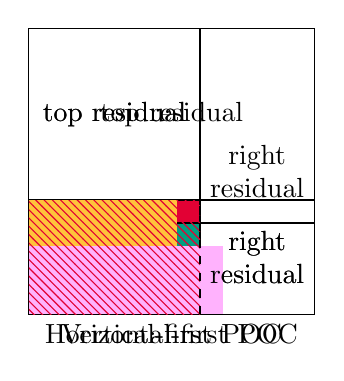
\begin{tikzpicture}[scale=0.145]
\def\piececolor{crimson}
\def\piececolorb{creepers}
\def\labelxshift{12.5}
\def\labelyshift{0}
\def\labelfontsize{\normalsize}
\begin{scope}[shift={(0, 0)}] % FIRST ROW
\begin{scope}[shift={(0, 0)}] % FIRST IMAGE

% PIECES (and piece label)

\onslide<3,5-9>{\fill[\piececolor] (0, 0) rectangle +(15, 10);}
\onslide<4>{\fill[\piececolorb] (0, 0) rectangle +(15, 8);}
\onslide<5-9>{\node [align=center, font=\labelfontsize\selectfont] at (7.5, 5) {\labelfontsize piece};} %{\labelfontsize piece-sized \\ \labelfontsize plate};

% HORIZONTAL-FIRST

\onslide<2-6,10>{\draw[thick, black] (0, 10) -- (25, 10);}
\onslide<4>{\draw[thick, black] (0, 8) -- (25, 8);}

\onslide<6,10>{\node [align=center, font=\labelfontsize\selectfont] at (12.5, 17.5) {\labelfontsize top residual};}

% these exist but below, so they are not covered
%\onslide<5,6,10>{\draw[dashed, thick, black] (15, 0) -- (15, 10);}
%\onslide<6,10>{\node [align=center, font=\labelfontsize\selectfont] at (20, 5) {right\\residual};}

\onslide<6,8,10>{\node [below] at (\labelxshift, \labelyshift) {\labelfontsize Horizontal-first POC};}

% VERTICAL-FIRST
\onslide<7>{\draw[thick, black] (15, 0) -- (15, 25);}
\onslide<7>{\draw[dashed, thick, black] (0, 10) -- (15, 10);}

\onslide<7>{\node [align=center, font=\labelfontsize\selectfont] at (7.5, 17.5) {\labelfontsize top residual};}
\onslide<7>{\node [align=center, font=\labelfontsize\selectfont] at (20, 12.5) {right\\residual};}

\onslide<7,9>{\node [below] at (\labelxshift, \labelyshift) {\labelfontsize Vertical-first POC};}

% THE FIRST SIZE ORIGINAL PLATE SIZE
\onslide<1-7,10->{\draw (0,0) rectangle +(25, 25);}

% THE SINGLE-CUT HORIZONTAL POC

\onslide<8>{\draw[thick, black] (0, 10) -- (15, 10);}
\onslide<8>{\draw (0,0) rectangle +(15, 25);}
\onslide<8>{\node [align=center, font=\labelfontsize\selectfont] at (7.5, 17.5) {\labelfontsize top residual};}

% The SINGLE-CUT VERTICAL POC

\onslide<9>{\draw[thick, black] (15, 0) -- (15, 10);}
\onslide<9>{\draw (0,0) rectangle +(25, 10);}
\onslide<9>{\node [align=center, font=\labelfontsize\selectfont] at (20, 5) {right\\residual};}

% THE EXCEPTION

\onslide<10>{\fill[plum] (0, 0) rectangle +(17, 6);}
\onslide<10>{\fill[spark] (0, 6) rectangle +(13, 4);}
\onslide<10>{\draw[draw=none, pattern=north west lines, pattern color=crimson] (0,0) rectangle +(15, 10);}
\onslide<5,6,10>{\draw[dashed, thick, black] (15, 0) -- (15, 10);}
\onslide<6,10>{\node [align=center, font=\labelfontsize\selectfont] at (20, 5) {right\\residual};}

\end{scope}
\end{scope}
\end{tikzpicture}

}

\subsection{Formulation}

\frame{\frametitle{Changes in the formulation (hybridisation)}
\begin{align*}
\bm{max.} &\sum_{(i, j) \in E} p_i e_{ij} \newthing{+ \sum_{i \in \bar{J}} p_i s_i}\\
\bm{s.t.} &\specialcell{\newthing{s_i +} \sum_{j \in E_{i*}} e_{ij} \leq u_i \hspace*{\fill} \forall i \in \bar{J},}\\
	    & \specialcell{\sum_{o \in O}\sum_{q \in Q_{0o}} x^o_{q0} + \sum_{i \in E_{*0}} e_{i0} \leq 1 \hspace*{\fill},}\\
            & \specialcell{\sum_{o \in O}\sum_{q \in Q_{jo}} x^o_{qj} + \sum_{i \in E_{*j}} e_{ij} \leq \sum_{k \in J}\sum_{o \in O}\sum_{q \in Q_{ko}} \textcolor{blue}{a^o_{qkj}} x^o_{qk} \hspace*{0.05\textwidth} \forall j \in J, j \neq 0,}\\
            & \specialcell{\newthing{s_i \leq \sum_{j \in J}\sum_{o \in O}\sum_{q \in Q_{jo}} h^o_{qji} x^o_{qj}} \hspace*{\fill} \newthing{\forall i \in \bar{J}.}}\\
\end{align*}
}

\subsection{Results}

\frame{\frametitle{Summary of our results (Hybridisation)}
\begin{itemize}
\item FMT59 dataset: the run time reduction was of 20\%.
\begin{itemize}
\item Runs with 99\%+ of the run time in the B\&B phase are the most affected.
\end{itemize}
\item Clautiaux42 dataset (high length/width piece repetition):
\begin{itemize}
\item If positions of shared piece length/width are ignored: -1.5\% run time.
\item If we create POCs for every possible piece: +236\% run time.
\end{itemize}
\end{itemize}
}


\mysection{Related problems}
\subsection{G2MKP}
\frame{\frametitle{Summary of the G2MKP characteristics}
\begin{itemize}
\item Knapsack -- maximises profit, \notanymore{single} \newthing{multiple equal} plates.
\item \sameasbefore{Guillotine Cuts -- from a side to another.}
\item \sameasbefore{Orthogonal Cuts -- only cuts parallel to the sides.}
\item \sameasbefore{Unrestricted Cuts -- may cut in any position.}
\item \sameasbefore{Constrained Demand -- upper bound for pieces in solution.}
\item \sameasbefore{Unlimited Stages -- no limit on cut orientation changes.}
\item \sameasbefore{Allow/disallow rotation -- of pieces or plates.}
\end{itemize}
}

\frame{\frametitle{Changes to the formulation (G2MKP)}
\begin{align*}
\bm{max.} & \sum_{(i, j) \in E} p_i e_{ij}\\
\bm{s.t.} & \specialcell{\sum_{j \in E_{i*}} e_{ij} \leq u_i \hspace*{\fill} \forall i \in \bar{J},}\\
          & \specialcell{\sum_{o \in O}\sum_{q \in Q_{0o}} x^o_{q0} + \sum_{i \in E_{*0}} e_{i0} \leq \notanymore{1}\newthing{m} \hspace*{\fill},}\\
          & \specialcell{\sum_{o \in O}\sum_{q \in Q_{jo}} x^o_{qj} + \sum_{i \in E_{*j}} e_{ij} \leq \sum_{k \in J}\sum_{o \in O}\sum_{q \in Q_{ko}} a^o_{qkj} x^o_{qk} \hspace*{0.05\textwidth} \forall j \in J, j \neq 0,}\\
\end{align*}
}

\frame{\frametitle{Summary of our findings G2MKP}
\begin{itemize}
\item Least studied of the chosen problems.
\item Different datasets have different behaviours:
\begin{itemize}
\item For the CW\_M dataset (low \(u_i\), high \(n\)):
\begin{itemize}
\item Increasing \(m\) increased the times (many timeouts). % hundreds to thousands of times
\item Allowing rotation increased time and model size (\(2.8\tilderange7.5\)). % smaller effect on time but also orders of magnitude
\end{itemize}
\end{itemize}
\begin{itemize}
\item For the A\_M dataset (high \(u_i\), low \(n\)):
\begin{itemize}
\item Increasing \(m\) increased times lightly (\(< 17\%\)).
\item Allowing rotation increased time and model size (many OOM).
\end{itemize}
\end{itemize}
\end{itemize}
}

% TODO: move to the right place
\subsection{G2CSP/G2BPP}
\frame{\frametitle{Summary of the G2CSP/G2BPP characteristics}
\begin{itemize}
\item \notanymore{Knapsack -- maximises profit, single plate.}
\item \newthing{Input minimisation -- minimises number of bins.}
\item \sameasbefore{Guillotine Cuts -- from a side to another.}
\item \sameasbefore{Orthogonal Cuts -- only cuts parallel to the sides.}
\item \sameasbefore{Unrestricted Cuts -- may cut in any position.}
\item \notanymore{Constrained Demand -- upper bound for pieces in solution.}
\item \newthing{Required Demand -- \emph{lower} bound for pieces in solution.}
\item \sameasbefore{Unlimited Stages -- no limit on cut orientation changes.}
\item \sameasbefore{Allow/disallow rotation -- of pieces or plates.}
\end{itemize}
}

\frame{\frametitle{Changes to the formulation (G2CSP/G2BPP)}
\begin{align*}
\notanymore{\bm{max.}} & \notanymore{\sum_{(i, j) \in E}} \notanymore{p_i e_{ij}}\newthing{\bm{min.}}~\newthing{b}\\
\bm{s.t.} & \specialcell{\sum_{j \in E_{i*}} e_{ij} \notanymore{\leq}\newthing{\geq} u_i \hspace*{\fill} \forall i \in \bar{J},}\\
          & \specialcell{\sum_{o \in O}\sum_{q \in Q_{0o}} x^o_{q0} + \sum_{i \in E_{*0}} e_{i0} \leq \notanymore{1}\newthing{b} \hspace*{\fill},}\\
          & \specialcell{\sum_{o \in O}\sum_{q \in Q_{jo}} x^o_{qj} + \sum_{i \in E_{*j}} e_{ij} \leq \sum_{k \in J}\sum_{o \in O}\sum_{q \in Q_{ko}} a^o_{qkj} x^o_{qk} \hspace*{0.05\textwidth} \forall j \in J, j \neq 0,}\\
\end{align*}
}

\frame{\frametitle{Summary of our findings (G2CSP/G2BPP)}
\begin{itemize}
\item Other methods have better results (but no direct comparison)
\begin{itemize}
\item Either not exact, tackle a simpler problem, or not pure MILP.
\end{itemize}
\item Different datasets have different behaviours:
\begin{itemize}
\item For the A dataset (high \(u_i\), low \(n\)):
\begin{itemize}
\item Allowing rotation almost always lead to OOM.
\end{itemize}
\end{itemize}
\begin{itemize}
\item For the CLASS dataset (low \(u_i\), high \(n\)):
\begin{itemize}
\item Allowing rotation generally reduced model size and run time.
\item Many pieces for small plate led to discretization saturation.
\item Better primals helped when model size did increase.
\end{itemize}
\end{itemize}
\end{itemize}
}


% TODO: move to the right place
\subsection{G2OPP}
\frame{\frametitle{Summary of the G2OPP characteristics}
\begin{itemize}
\item \notanymore{Knapsack -- maximises profit,} single plate.
\item \newthing{Decision problem -- checks feasibility of packing all pieces.}
\item \sameasbefore{Guillotine Cuts -- from a side to another.}
\item \sameasbefore{Orthogonal Cuts -- only cuts parallel to the sides.}
\item \sameasbefore{Unrestricted Cuts -- may cut in any position.}
\item \notanymore{Constrained Demand -- upper bound for pieces in solution.}
\item \newthing{Required Demand -- \emph{lower} bound for pieces in solution.}
\item \sameasbefore{Unlimited Stages -- no limit on cut orientation changes.}
\item \sameasbefore{Allow/disallow rotation -- of pieces or plates.}
\end{itemize}
}

\frame{\frametitle{Changes to the formulation (G2OPP)}
\begin{align*}
\notanymore{\bm{max.}} & \notanymore{\sum_{(i, j) \in E}} \notanymore{p_i e_{ij}}\\
\bm{s.t.} & \specialcell{\sum_{j \in E_{i*}} e_{ij} \notanymore{\leq}\newthing{\geq} u_i \hspace*{\fill} \forall i \in \bar{J},}\\
          & \specialcell{\sum_{o \in O}\sum_{q \in Q_{0o}} x^o_{q0} + \sum_{i \in E_{*0}} e_{i0} \leq 1 \hspace*{\fill},}\\
          & \specialcell{\sum_{o \in O}\sum_{q \in Q_{jo}} x^o_{qj} + \sum_{i \in E_{*j}} e_{ij} \leq \sum_{k \in J}\sum_{o \in O}\sum_{q \in Q_{ko}} a^o_{qkj} x^o_{qk} \hspace*{0.05\textwidth} \forall j \in J, j \neq 0,}\\
\end{align*}
}

\frame{\frametitle{Summary of our findings (G2CSP/G2BPP)}
\begin{itemize}
\item Competitive against CP, but not against an \emph{ad hoc} method.
\begin{itemize}
\item The \emph{ad hoc} has a memory complexity of \(2(min\{W,L\}2^n)^2\)
\end{itemize}
\item Allowing rotation increases model size but reduces run times.
\item The run time decrease relates to instances becoming feasible.
\item Mirror-plate is able to reduce model size and run time.
\end{itemize}
}

\frame{\frametitle{About the T instances from Hopper (2000)}
\begin{itemize}
\item We found a dataset generation mistake during experiments.
\item For the G2OPP, \emph{all} T instances should return true.
\begin{itemize}
\item However, it seems all return false.
\end{itemize}
\item Some works may have been impacted: \cite{bortfeldt:2012,thomas:2014,shang:2020}.
\item The mistake was (probably) to use the same procedure of dataset N.
\end{itemize}
}

\frame{\frametitle{A non-guillotinable optimal solution for instance T1a}
\begin{figure}[h]
  \center
  \includegraphics[width=0.6\linewidth]{T1a.pdf}
  \label{fig:T1a}
\end{figure}
}

\mysection{Conclusions}
\frame{\frametitle{Conclusions}
\begin{itemize}
\item The (re-)formulation and PSN show an order of magnitude improvement.
\begin{itemize}
\item For instances that can be solved with MILP, solves the most.
\item For harder instances, fail to deliver good primal solutions.
\end{itemize}
\item Hybridisation further reduces time spent on B\&B by 20\%.
\item For related problems, \emph{ad hoc} methods have the advantage.
\begin{itemize}
\item However, a direct comparison is hard in most cases.
\item Our work may serve as base for future comparisons.
\end{itemize}
\end{itemize}
}

\begin{frame}[c]{Conclusions II}
\center
Breaking symmetries and removing dominated variables had better results than resorting to more complicated variable pricing techniques.\\[1cm]
These improvements are immediately compatible with related problems, and do not depend on problem-specific heuristics like some pricing techniques.
\end{frame}

\begin{frame}[c]{}
\center
\Huge Thank you all.
\end{frame}

\bibliographystyle{splncs03}

\backupbegin
\setbeamertemplate{footline}{}
\begin{frame}[allowframebreaks]{References}
\small
\bibliography{thesis_slides}
\end{frame}
\backupend
\end{document}

